\documentclass[10pt, a4paper]{article} % 设置字体大小和纸张类型
\usepackage{fontspec}
\setmainfont{Times New Roman}

\usepackage{booktabs} % 支持更专业的表格线条
\usepackage{ctex}
\usepackage{caption} % 插图和表格的标题格式
\usepackage{amsmath, amsfonts, amssymb} % 数学公式支持
\usepackage{graphicx} % 插入图片
\usepackage{hyperref} % 超链接支持
\usepackage{hypcap} % 修正超链接指向的图片位置
\usepackage[a4paper, margin=1in]{geometry}
\usepackage{titlesec}
\usepackage{fmtcount} % 用于数字到中文的转换
\usepackage{enumitem} % 加载 enumitem 宏包
\usepackage{multirow} % 支持多行单元格
\usepackage{diagbox}
\usepackage{makecell} % 支持单元格内换行
\usepackage{tikz}
\usepackage{makecell}
\usepackage{unicode-math}
\usepackage{bookmark} % 书签支持
\setmathfont{Latin Modern Math}



\renewcommand{\thesection}{\chinese{section}、}
\renewcommand{\thesubsection}{\arabic{subsection}.}


\begin{document}

\begin{titlepage}
    \newgeometry{left=0cm, right=0cm, top=0cm, bottom=0cm}
    \centering
    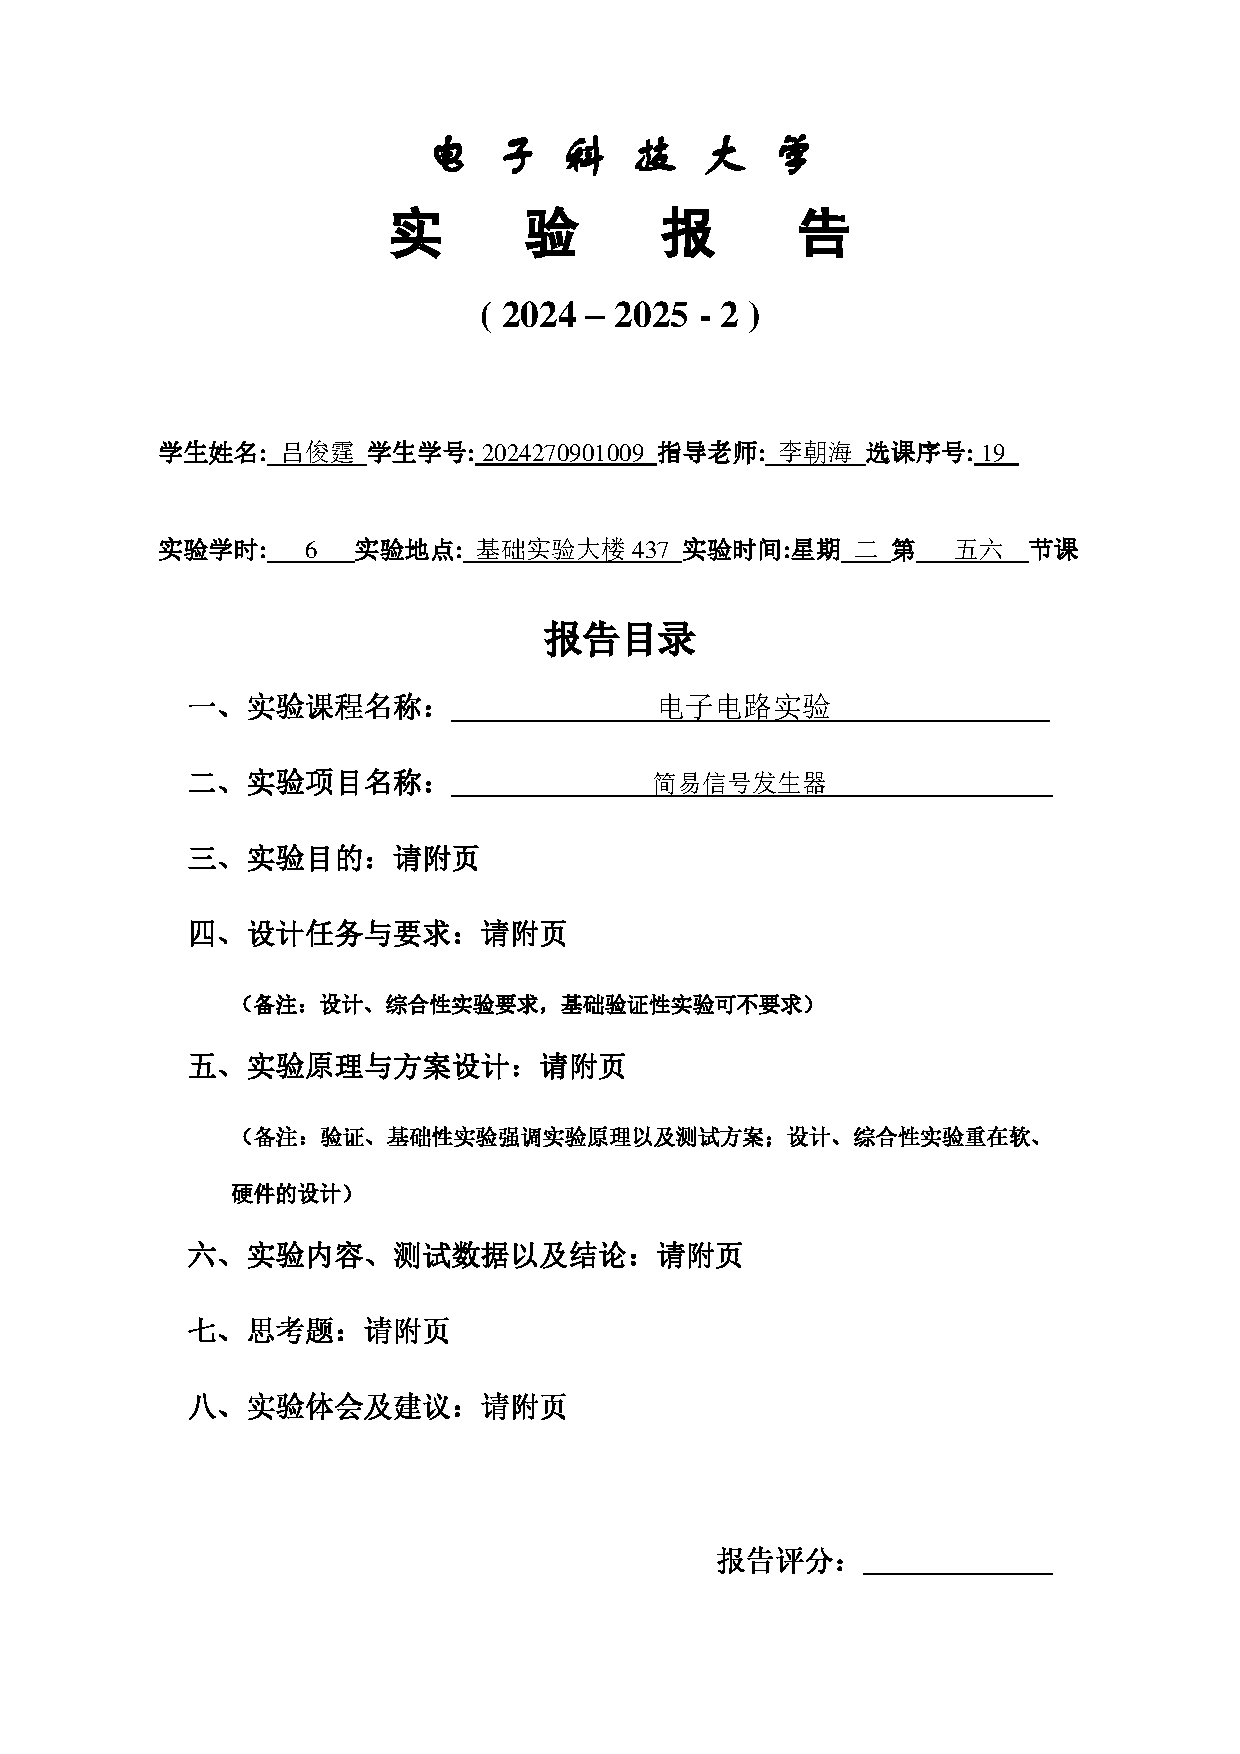
\includegraphics[page=1, width=0.9\textwidth, keepaspectratio]{image/实验报告撰写封面.pdf}
    \restoregeometry
\end{titlepage}

\setcounter{section}{2}

\section{实验目的}

\begin{enumerate}[leftmargin=50pt,label=(\arabic*)] % 设置序号格式为(1)
    \item 了解文氏桥RC正弦波产生电路设计原理。
    \item 了解电压比较器电路设计原理。
    \item 了解积分器电路设计原理
\end{enumerate}

\section{设计任务与要求}

产生正弦波信号,通过正弦波信号进行比较器设计,输出方波信号,再通过设计合适的时间常数,利用积分器电路实现方波到三角波的波形转换。

\section{实验原理与方案设计}
\subsection{实验原理}
\subsubsection{文氏桥RC正弦波产生电路原理}
文氏桥振荡器是一种常用的正弦波振荡电路,主要由运算放大器和RC网络组成。其基本原理是利用RC网络的相位移特性和运算放大器的增益特性来实现自激振荡。文氏桥振荡器的输出信号为正弦波,频率由RC网络的时间常数决定。
文氏桥的原理电路和实验电路如下图所示:
\begin{figure}[th]
    \centering
    \begin{minipage}{0.45\textwidth}
        \centering
        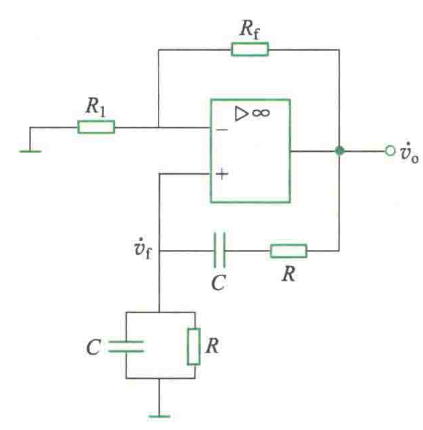
\includegraphics[width=\textwidth]{image/1.png}
        \caption{文氏桥原理电路}
        \label{fig:文氏桥原理电路}
    \end{minipage}
    \hfill
    \begin{minipage}{0.45\textwidth}
        \centering
        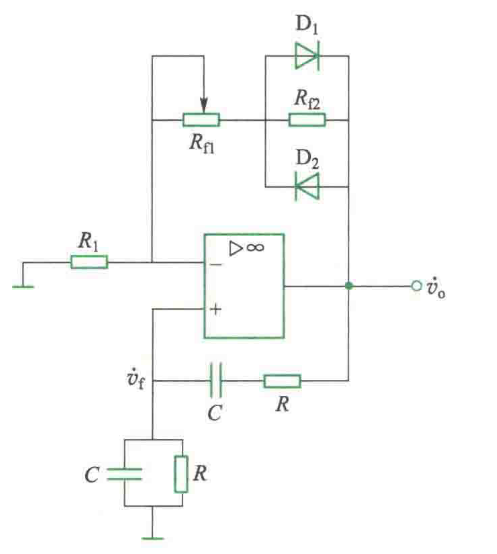
\includegraphics[width=\textwidth]{image/2.png}
        \caption{文氏桥实验电路}
        \label{fig:文氏桥实验电路}
    \end{minipage}
    
\end{figure}

正弦波振荡电路的构成必须包括四个组成部分,
第一部分是放大电路,它保证电路能起振,使输出经历由小到大直到稳幅的动态平衡过程。
第二部分是正反馈网络,它使放大电路的输入信号等于反馈信号。
第三部分是选频网络,它确保只对单一频率进行正反馈,这样其他频率的输出量逐渐衰减到零,电路就产生单一频率的振荡,即正弦波振荡。
第四部分是稳幅环节,它利用器件的非线性使输出信号的幅值稳定。在实用电路中常将正反馈网络和选频网络合二为一。
正弦波振荡电路常分为 RC 正弦波振荡电路、LC 正弦波振荡电路和石英晶体正弦波振荡电路几种。
其中 RC 正弦波振荡电路适用于振荡频率较低的应用场合。

图~\hyperref[fig:文氏桥原理电路]{\ref{fig:文氏桥原理电路}}所示是最具典型性的 RC 正弦波振荡电路——RC 文氏桥振荡电路。其中,放大电路选用输入电阻大且输出电阻小的同相比例运算放大电路,以降低输入电阻和输出电阻对选频特性的影响。正反馈网络和选频网络是合二为一的,由 RC 串并联选频网络来担任,反馈系数为


\begin{align}
    \beta = \frac{R // \frac{1}{j\omega C}}{R + \frac{1}{j\omega C} + R // \frac{1}{j\omega C}} = \frac{R // \frac{1}{j\omega C}}{R + 2R // \frac{1}{j\omega C}}
\end{align}
\label{eq:反馈系数}

令 $f_0 = \frac{1}{2\pi RC}$,则


 $$
\dot{F} = \frac{\dot{v}_f}{\dot{v}_o} = \frac{1}{3 + j\left(\frac{f}{f_0} - \frac{f_0}{f}\right)}
$$ 

当 $f = f_0$ 时,$\dot{F} = \frac{1}{3}$,根据平衡条件,要求 $\dot{A} = 3$。同相比例运算放大器的放大倍数为(不接二极管并联稳幅支路时)


 $$
\dot{A} = \frac{\dot{v}_o}{\dot{v}_i} = 1 + \frac{R_f}{R_1}
$$ 

即需满足 $R_f = 2R_1$。起振条件为 $|\dot{A}\dot{F}| > 1$,故 $R_f$ 的取值要略大于 $2R_1$。

最后,需要一个稳幅环节。运算放大器输出受饱和和输出电压的限制,如果依靠饱和输出电压来稳幅的话,输出会有明显失真,所以一般在电路中加入非线性器件,如热敏电阻、二极管,来稳定输出电压的幅值。

\subsubsection{电压比较器电路原理}
电压比较器是将输入的模拟信号与参考电压进行比较,输出高低电平信号的电路。其基本原理是利用运算放大器的差分输入特性,将输入信号与参考电压进行比较,当输入信号大于参考电压时,输出高电平;当输入信号小于参考电压时,输出低电平。

(1)过零比较器

过零比较器稍加变动,就可以构成阈值不为零的其他单限比较器,这类比较器的作用是用来检测输入的模拟信号是否达到某一给定的电平,但这类比较器有一个明显的缺点,就是抗干扰能力差,输入电压由于噪声干扰在阈值电压附近有微小的变化,都会引起输出电压的跃变。解决的办法就是采用具有滞回传输特性的比较器。

\begin{figure}[htbp]
    \centering
    \begin{minipage}{0.45\textwidth}
        \centering
        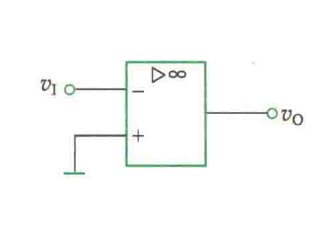
\includegraphics[width=\textwidth]{image/3.png}
        \caption{过零比较器}
    \end{minipage}
    \hfill
    \begin{minipage}{0.45\textwidth}
        \centering
        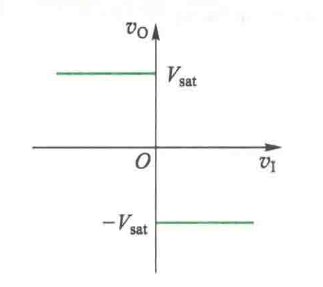
\includegraphics[width=\textwidth]{image/4.png}
        \caption{过零比较器电压传输特性}
    \end{minipage}
    \caption{过零比较器电路及电压传输特性}
    \label{fig:zero_crossing}
\end{figure}

(2)滞回比较器

滞回比较器又称迟滞比较器。如图 \ref{fig:hysteresis}(a) 所示电路是一个反相输入端作为输入的滞回比较器电路。运放的输出为正或负的饱和输出电压,通过正反馈后,同相输入端的电压可通过分压比获得。令反相输入端电压等于同相输入端电压,求出的输入电压即为阈值电压。如果假设正的饱和输出电压和负的饱和输出电压相等,则阈值电压分别为 $+V_T$ 和 $-V_T$。

\begin{figure}[htbp]
    \centering
    \begin{minipage}{0.45\textwidth}
        \centering
        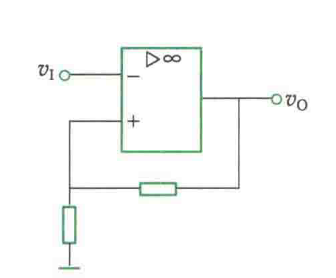
\includegraphics[width=\textwidth]{image/5.png}
        \caption{滞回比较器电路}
    \end{minipage}
    \hfill
    \begin{minipage}{0.45\textwidth}
        \centering
        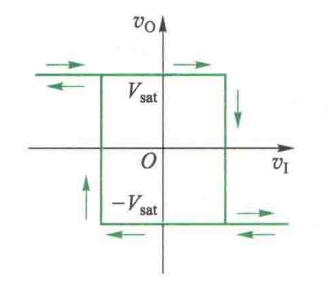
\includegraphics[width=\textwidth]{image/6.png}
        \caption{滞回比较器电压传输特性}
    \end{minipage}
    \caption{滞回比较器电路及电压传输特性}
    \label{fig:hysteresis}
\end{figure}

如果输入电压 $v_1 < -V_T$,那么因为同相端电压比反相端电压大,输出为正的饱和输出电压 $+V_{\text{sat}}$,反馈到同相端,则此时的阈值电压为正的 $+V_T$。只有输入电压从小于 $-V_T$ 增大到大于 $+V_T$,反相端输入电压比同相端输入电压大时,输出才会由正的饱和输出电压 $+V_{\text{sat}}$ 变为负的饱和输出电压 $-V_{\text{sat}}$,同相端输入电压变为 $-V_T$。

如果输入电压 $v_1 > V_T$,当反相端输入电压减小时,由于此时同相端输入电压变为 $-V_T$,所以反相端输入电压经过阈值电压 $+V_T$ 时,输出并不会跃变,而是直到达到阈值电压 $-V_T$ 时,输出才会由负的饱和输出电压 $-V_{\text{sat}}$ 跃变为正的饱和输出电压 $+V_{\text{sat}}$。由于电压传输特性呈现出一定的惯性,所以具有一定的抗干扰能力。

\subsubsection{积分器电路原理}
积分器电路是将输入信号进行积分运算,输出与输入信号的积分值成正比的电路。其基本原理是利用运算放大器的反馈特性,将输入信号进行积分运算。积分器电路的输出信号为三角波,频率由输入信号的频率和反馈电阻的大小决定。

(1) 理想积分器

由于电容中的电流与其电压对时间的变化率成正比,所以电容上的电压等于其电流的积分。根据这个特性,可以用运算放大器构成如图 6.5.1(a)所示的理想积分器。其中,集成运放的反相输入端为“虚地”,电容  $ C $  中的电流  $ i_C $  等于电阻  $ R $  中的电流  $ i_R $ 。输出电压  $ v_o $  和输入电压  $ v_i $  借助电容上的电压  $ v_C $  形成积分关系


 $$
v_o = -v_C = -\frac{1}{C} \int i_C \, \mathrm{d}t = -\frac{1}{C} \int \frac{v_i}{R} \, \mathrm{d}t = -\frac{1}{RC} \int v_i \, \mathrm{d}t
$$ 

如果求解  $ t_1 $  到  $ t_2 $  时间段的积分值,输出电压可以表示为


 $$
v_o = -\frac{1}{RC} \int_{t_1}^{t_2} v_i \, \mathrm{d}t + v_o(t_1)
$$ 

其中  $ v_o(t_1) $  是积分起始时刻的输出电压。 $ \tau = RC $  称为积分时间常数。

(2) 实际积分器
由于实际运算放大器、实际电容器与理想运算放大器、理想电容器的差异,实际积分器与理想积分器相比,会产生多项误差。

对于集成运放来说,输入失调电压和偏置电流在这个电路中会持续地使积分电容累积电荷,即使积分器在零输入的情况下,运放的输出电压相应地连续向一个方向改变,最终积分器的输出将漂移至正的或者是负的饱和状态,形成积分漂移现象。另一方面,有限的开环增益、输入阻抗和带宽也会带来非线性失真的问题。对于电容器来说,泄漏电阻和介质损耗都会带来积分误差。

解决措施首先是要挑选失调电压、偏置电流、增益带宽等各方面参数好的集成运放以及质量好的优质电容。对于积分漂移,可以在积分电容两侧并联一个合适的电阻,如图 6.5.1(b)所示。因为这个反馈电阻的存在,限制了低频,尤其是直流时的增益,这样,失调电压引起的漂移得到钳制,使输出不至于进入饱和而产生失真。

但是,接入  $ R_f $  后,反馈网络形成一个  $ RC $  网络,电流  $ i_R $  通过这个  $ RC $  网络使输出电压呈现指数变化特性,偏离了理想的积分特性。为了减小并联电阻  $ R_f $  对积分器的影响,在满足特定直流漂移要求的情况下应尽可能地选择大阻值  $ R_f $ 。

\begin{figure}[htbp]
    \centering
    \begin{minipage}{0.45\textwidth}
        \centering
        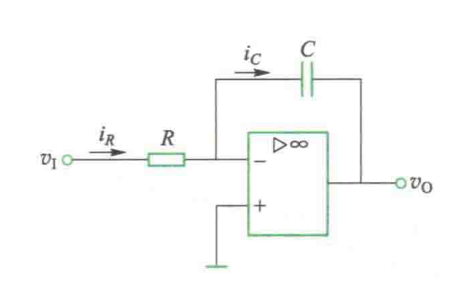
\includegraphics[width=\linewidth]{image/7.png}
        \caption{理想积分器}
        \label{fig:ideal_integrator}
    \end{minipage}\hfill
    \begin{minipage}{0.45\textwidth}
        \centering
        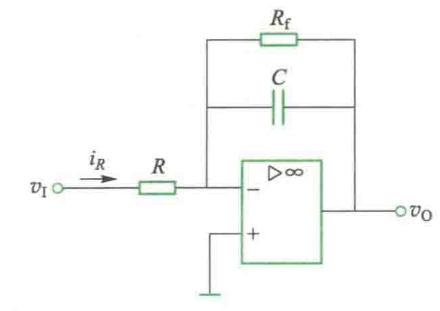
\includegraphics[width=\linewidth]{image/8.png}
        \caption{实际积分器电路}
        \label{fig:actual_integrator}
    \end{minipage}
    \caption{积分器电路}
    \label{fig:integrator}
\end{figure}


但是,接入  $ R_f $  后,反馈网络形成一个  $ RC $  网络,电流  $ i_R $  通过这个  $ RC $  网络使输出电压呈现指数变化特性,偏离了理想的积分特性。为了减小并联电阻  $ R_f $  对积分器的影响,在满足特定直流漂移要求的情况下应尽可能地选择大阻值  $ R_f $ 。



\section{实验内容、测试数据以及结论}

\subsection{实验内容}

\subsubsection{文氏桥RC正弦波产生电路实验}
\begin{enumerate}[leftmargin=50pt,label=(\arabic*)] % 设置序号格式为(1)
    \item 连接文氏桥RC正弦波产生电路,调整电位器,观察输出波形。
    \item 测量输出波形的频率和幅值,并记录数据。
\end{enumerate}
\subsubsection{电压比较器实验}
\begin{enumerate}[leftmargin=50pt,label=(\arabic*)] % 设置序号格式为(1)
    \item 连接电压比较器电路,调整输入信号幅值和参考电压。
    \item 测量输出波形的频率和幅值
    \item 观察滞回比较器的输出波形
\end{enumerate}

\subsubsection{积分器电路实验}
\begin{enumerate}[leftmargin=50pt,label=(\arabic*)] % 设置序号格式为(1)
    \item 连接积分器电路
    \item 观察输出波形的频率和幅值
\end{enumerate}
\subsection{实验结论}
实验结果如图
\begin{figure}[ht]
    \centering
    \begin{minipage}{0.23\textwidth}
        \centering
        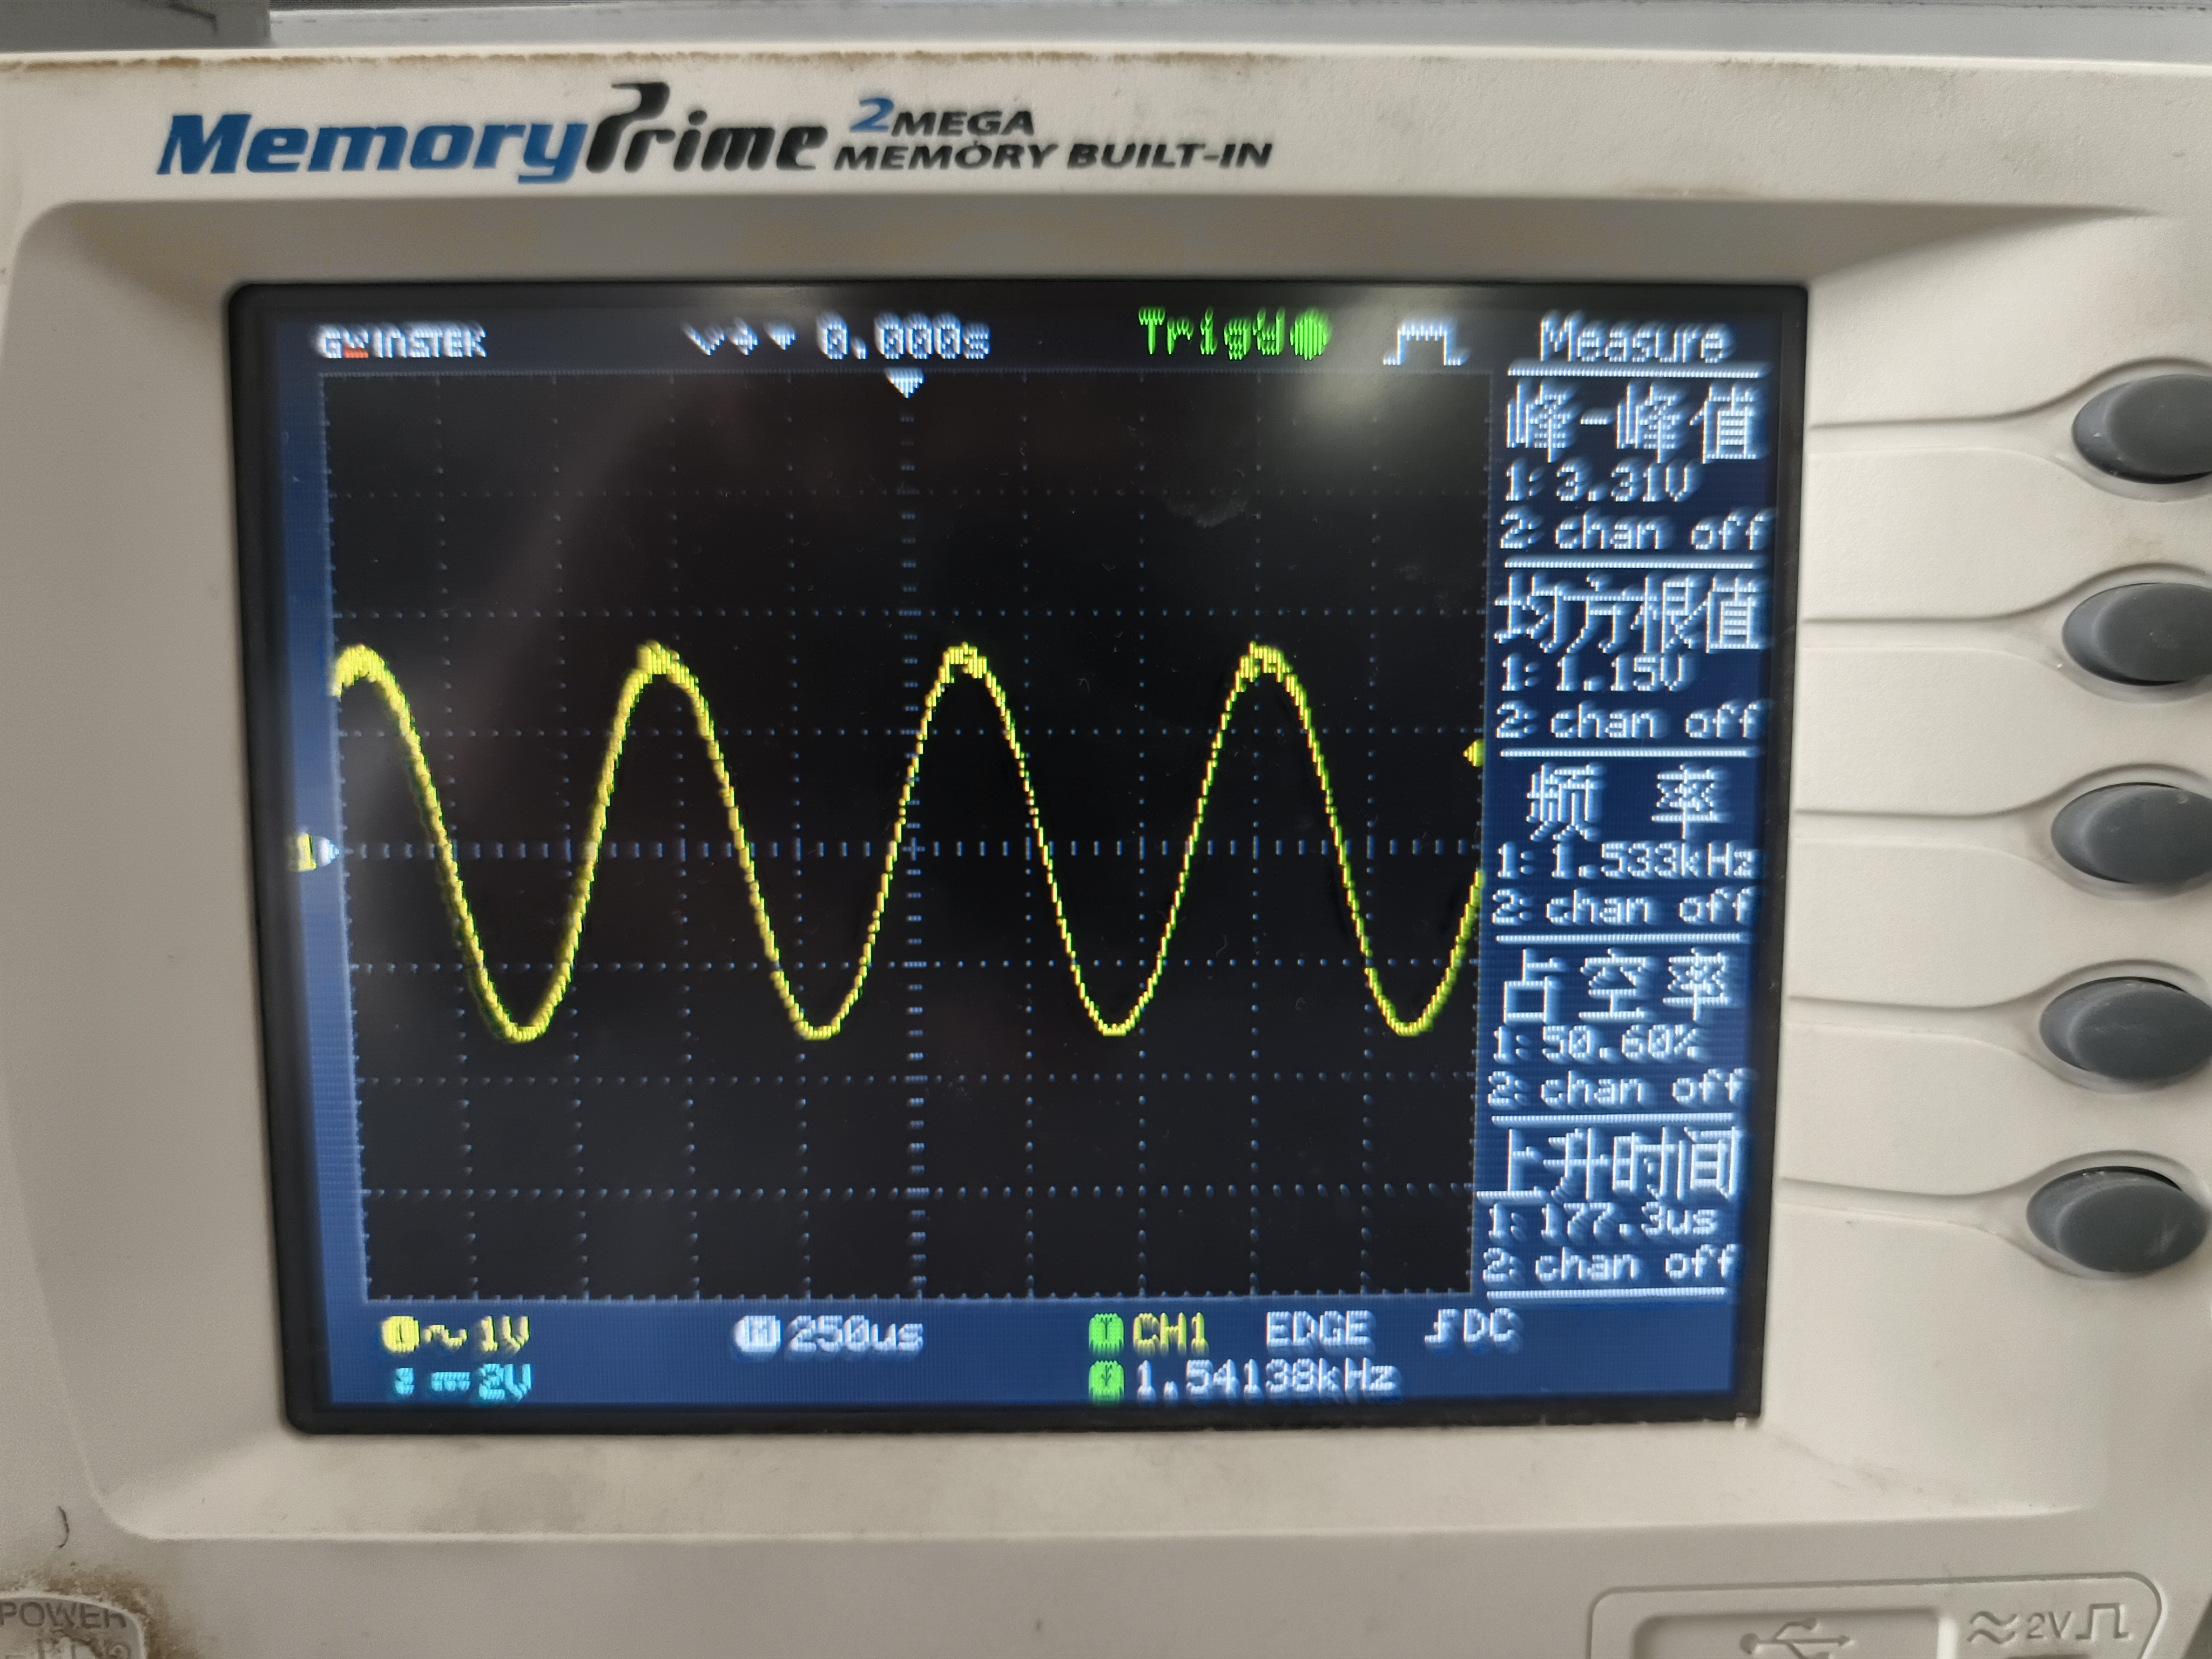
\includegraphics[width=1.0\textwidth]{image/9.jpg}
        \caption{文氏桥输出波形}
        \label{fig:文氏桥输出波形}
    \end{minipage}
    \hfill
    \begin{minipage}{0.23\textwidth}
        \centering
        \includegraphics[width=1.0\textwidth]{image/10.jpg}
        \caption{过零电压比较器输出波形}
        \label{fig:电压比较器输出波形}
    \end{minipage}
    \hfill
    \begin{minipage}{0.23\textwidth}
        \centering
        \includegraphics[width=1.0\textwidth]{image/11.jpg}
        \caption{滞回电压比较器输出波形}
        \label{fig:滞回电压比较器输出波形}
    \end{minipage}
    \hfill
    \begin{minipage}{0.23\textwidth}
        \centering
        \includegraphics[width=1.0\textwidth]{image/12.jpg}
        \caption{积分器输出波形}
        \label{fig:积分器输出波形}
    \end{minipage}

\end{figure}
\section{思考题}
\subsection{题面}
\begin{enumerate}[leftmargin=50pt,label=(\arabic*)] % 设置序号格式为(1)
    \item 文氏桥 RC 振荡器中,和二极管并联的电阻的作用是什么?
    \item 在滞回比较器中,如果输入正弦波的频率一直升高,则输出会是什么样的波形?是什么原因造成的?
    \item 在滞回比较器中,如何修改电路使比较器的输出电压改变?
    \item 积分器电路中,如果输入方波频率很低,则电路将实现什么功能?
    \item 分析实际积分器的误差来源。

\end{enumerate}
\subsection{回答}

\begin{enumerate}[leftmargin=50pt,label=(\arabic*)] % 设置序号格式为(1)
    \item 减小波形失真,稳定输出幅值。
    \item 在滞回比较器中,如果输入正弦波的频率一直升高,输出波形将会变成一系列越来越窄的脉冲波形,因为当输入信号频率升高时,比较器的输出会在两个阈值电压之间快速切换,导致输出波形的脉冲宽度变窄。
    \item 调整比较器的阈值电压
    \item 当输入方波频率很低时,积分器电路将实现低通滤波的功能。这意味着电路将允许低频信号通过,同时衰减高频信号。具体来说,输入的低频方波将被积分成近似的三角波,而方波中的高频成分将被大幅衰减。
    \item 运算放大器的非理想特性,电容的非理想特性,电阻的非理想特性,电源电压的波动等都会影响输出波形的稳定性和准确性。
\end{enumerate}

\section{实验体会及建议}
\subsection{实验体会}
测量时应注意小心调试仪器, 尽量将读数稳定在误差允许范围内进行读数。
\subsection{建议}
注意电源正负极的接入, 防止反接造成仪器损坏, 注意正负电压的接入, 防止反接造成仪器损坏。

\end{document}
